\documentclass[12pt]{article}

\usepackage{cite}
\usepackage{amstext}
\usepackage{amssymb}
\usepackage{amsmath}
%\usepackage{amssymb}
\usepackage{epsfig}
\usepackage{graphics}
\usepackage{graphicx}

\DeclareMathOperator\erf {erf}


\bibliographystyle{plain}

\begin{document}

\begin{titlepage}

\vfill \LARGE
\begin{center}
Convergence, Parker and Burton System
\large

\rule{0mm}{20mm}

O. J.  Halliday, S. D. Griffith,  D. Parker,

 \vspace{3mm} {\em University of Leeds}


%\rule{40mm}{0.2mm}



\end{center}

\pagestyle{empty}
\end{titlepage}
%
%
%
\section{Limits of Spatial-Temporal Convergence }
\label{sec_background}
%
We aim to study the convergence of our forced forced, lidded system of Parker and Burton, with transient heating function:
%
\begin{equation}
\frac{Q(x,z,t)}{Q_0}= \sin \left( \frac{\pi z }{ H_t} \right) ( H(t) - H(t-T)) ( H(z) - H(z-H_t)) F(x),
\end{equation}
%
where:
%
%
\begin{equation}
F(x) = \sigma_0 \sigma \exp \left( - \frac{x^2}{2 \sigma_0^2 \sigma^2 }\right), \quad 0<z<H_L.
\end{equation}
%
In particular, we wish to find approximate limits (bounds) on the spatial domain and timescales, implicitly imposed by our use of a rigid lid upper boundary condition.
 
The partial Fourier spectrum of the above function:
%
\begin{equation}
\label{equ_partial}
\frac{Q(x,z,t)}{Q_0} =  ( H(t) - H(t-T))  \sum_{m=1}^M  b_m \sin \left( \frac{ m \pi }{ H_L} z \right) ,
\end{equation}
%
where:
%
\begin{equation}
b_m =  \frac{2 \bar{H_t} \pi \sin \left( \bar{H_t} \pi \right) }{ 1 - \bar{H_t}^2 m^2 }, \quad \bar{H_t} = \frac{H_t}{H_L} , \quad M \propto H_L,
\end{equation}
%
is represented in figure \ref{fig_1} below, for $H_L =30 H_t$, $\sigma = 1$. Here, to ensure convergence, the number of Fourier modes $M$ used to express the above
function scales with lid height$H_L$. The choice of lid location, relative to the top of heating, ensures convergence in the $w$-response to approximately one per-cent. 

Let us denote the harmonic number of the Fourier series term in equation \ref{equ_partial} with largest $|b_m|$ as $m_{max}$. For the data in figure \ref{fig_1} we find:
find:
%
\begin{equation}
m_{max} = 23, \quad b_{m_{max}} = 0.035. 
\end{equation}
%
%
%
\begin{figure}[h]
\caption{Convergence data. The Fourier spectrum of the heating function and the variation with $z$ of the partial summation in equation \ref{equ_partial}. } 
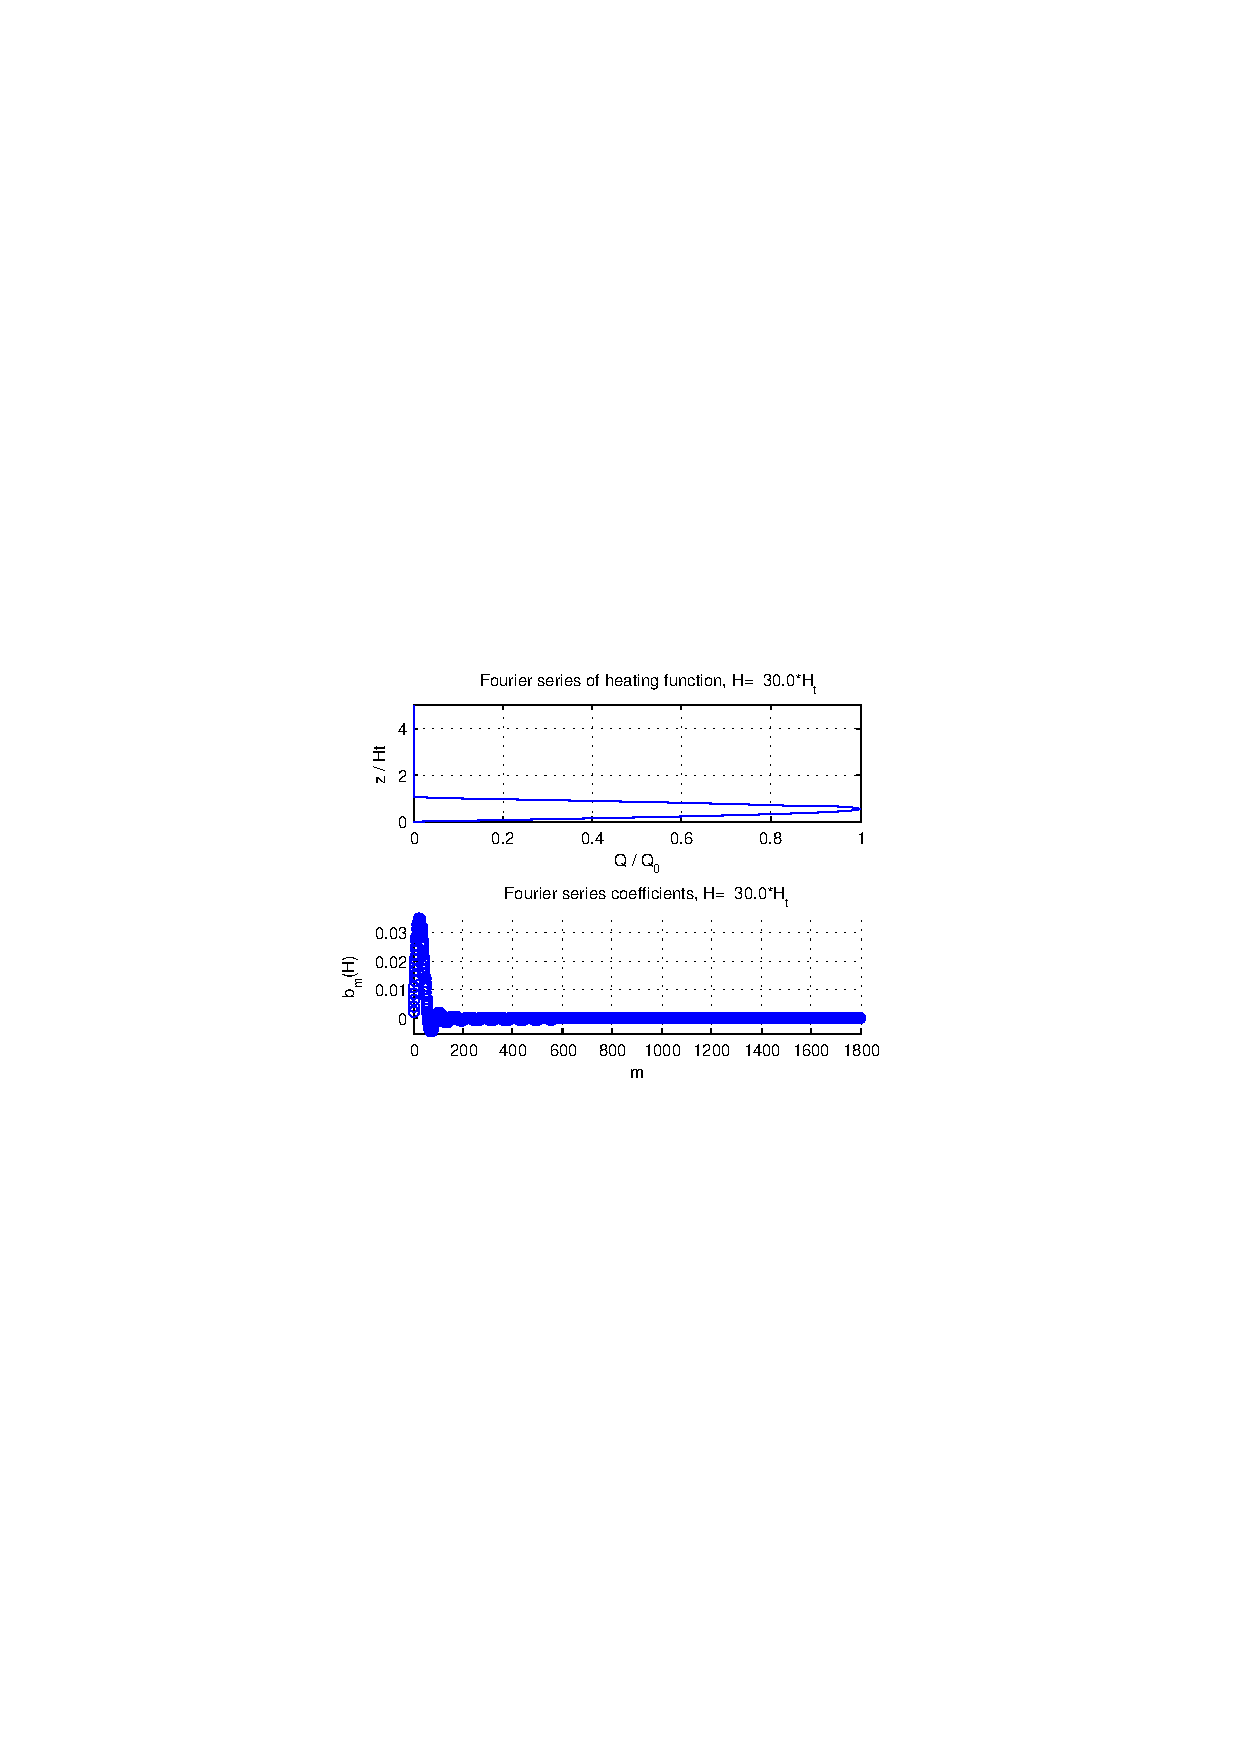
\includegraphics[scale=1.0,angle=-0] {fig1.pdf} 
\label{fig_1}
\end{figure}
%
%
%
We observe that the $w$-response is comprised of bores of vertical velocity perturbation which propagate approximately radially, from the fixed source of heat to the right 
as they elongate radially, weaken and descend. This response is apparent in a plot of the logarithm of the $w$-response in figure \ref{fig_2} below. 
%
%
%
\begin{figure}[h]
\caption{The $w$-response. Left panel is $\log_e(|w|)$, right panel $w$. The radial bores are visible in the plot on the left: the principal contribution is more clear on the light. 
The subset of $b_m$, $m<200$ are mainly responsible for each the features in the panel on the right. } 
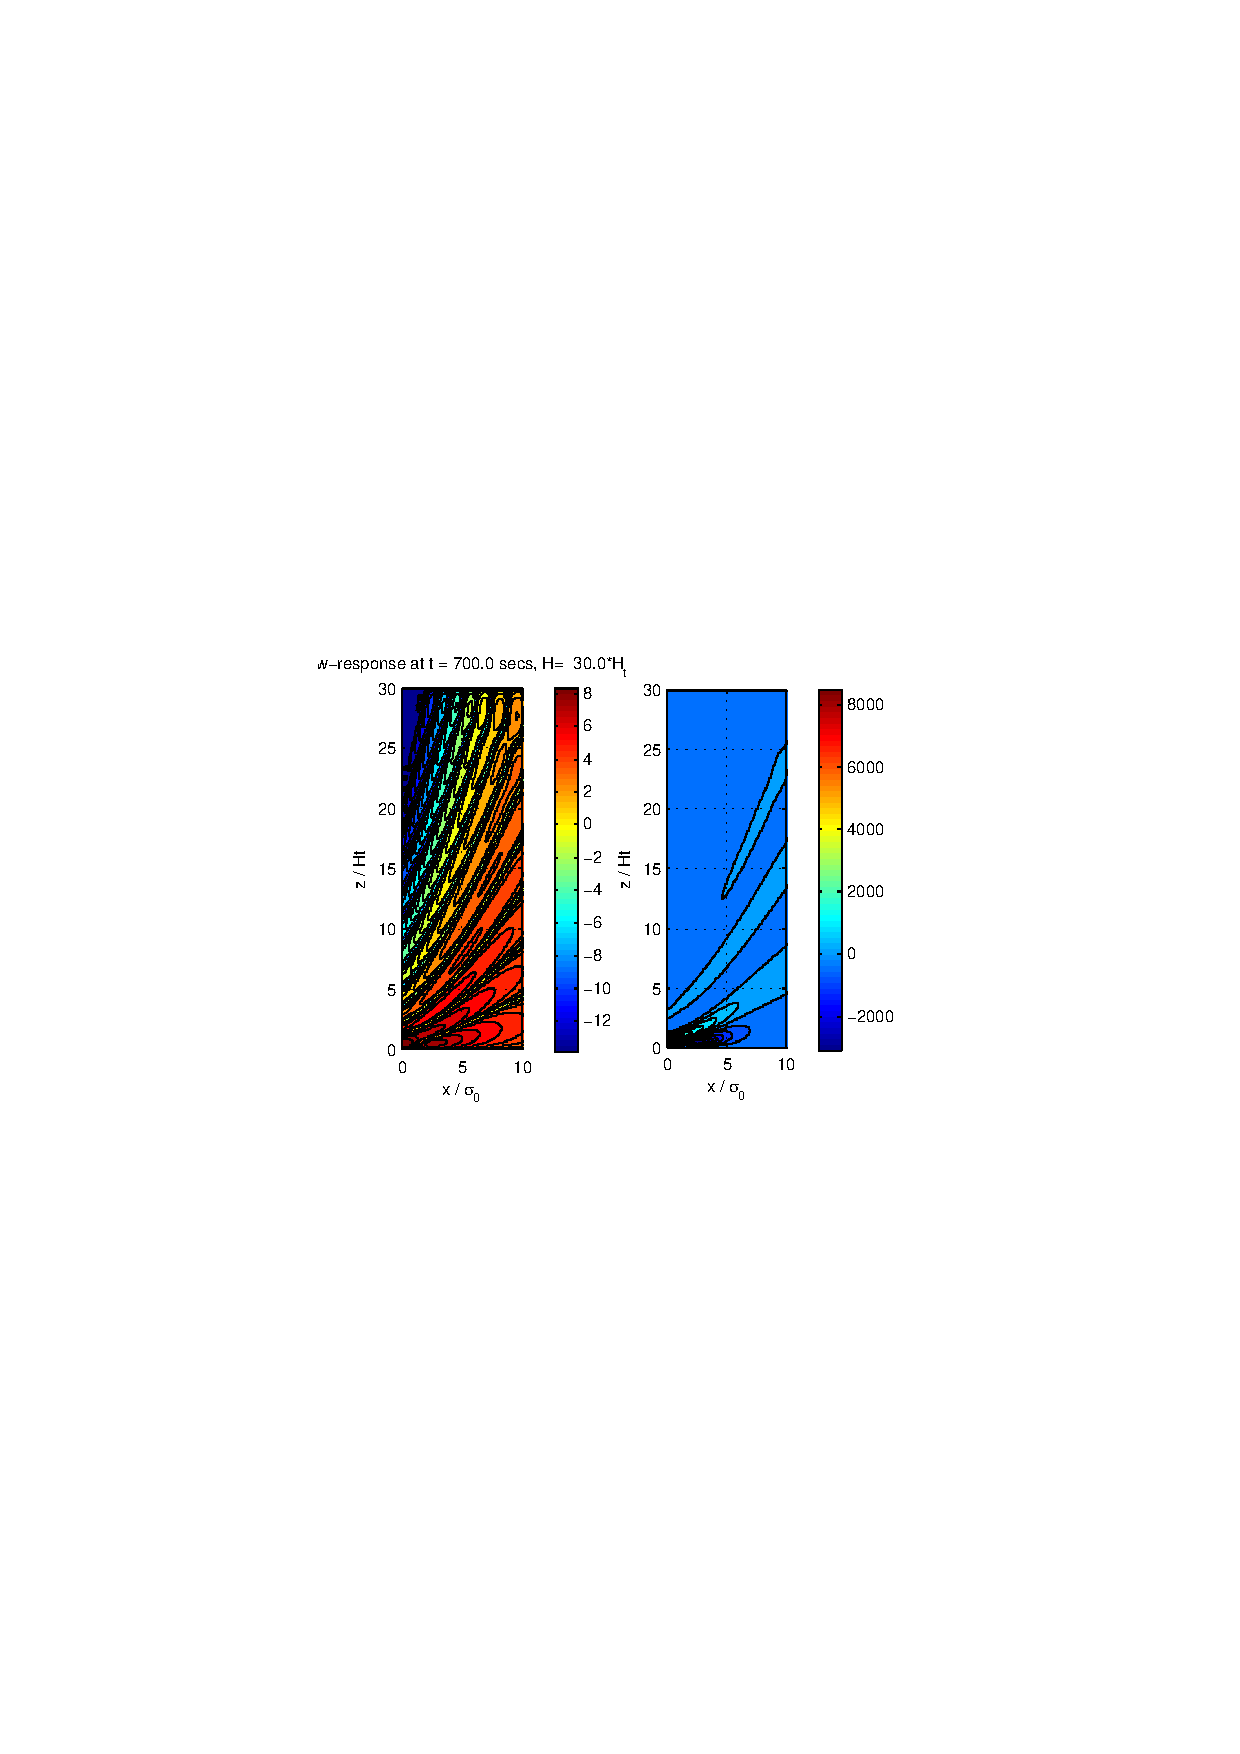
\includegraphics[scale=1.0,angle=-0] {fig2.pdf} 
\label{fig_2}
\end{figure}
%
%
%
Let us consider only the principal bores which may be attributed to the subset of modes $m < 200$, that is to those modes which contribute most strongly to the Fourier spectrum.

Let us model the motion of the strongest bores on freely propagating gravity waves in our slab system, characterized by a vertical wavelength (wavenumber) $\lambda_z$ ( $k_z$ ).
We obtain an extimate of this wavelength by considering the largest Fourier series term, namely $b_m \sin \left( \frac{ m_{max} \pi z }{ H_L}\right)$, which has a 
wavelength:
%
\begin{equation}
\label{equ_1}
\lambda_z \approx \frac{H_L}{m_{max} \pi } \iff k_z = \frac{2 \pi }{\lambda_z} = \frac{ 2 m_{max} }{ H_L }.
\end{equation}
%
The horizontal wavelength and wavevector of the principal bores must also be estimated. We take the FWHM of the horizontal variation of heating, $F(x)$:
%
\begin{equation}
\label{equ_2}
\lambda_x = \sigma \sigma_0 \iff k_x = \frac{2 \pi}{ \lambda_x} = \frac{2 \pi }{\sigma \sigma_0}.
\end{equation}
%
The above wavevector components are taken to be characteristic of the forced response in the Parker and Burton system. 

Now, the group and phase velocity of our assumed heat-induced Boussinesq gravity waves is determined from the appropriate dispersion relation for free modes of the 
Parker and Burton system [GAFD equ 2.32]:
%
\begin{equation}
\underline{c_g} = \pm \frac{N k_z}{( k_x^2 + k_z^2)^{3/2}} ( k_z,0,-k_x), \quad \underline{c_p} =   \frac{N }{k_x^2 + k_z^2} ( k_x,0,k_z),
\end{equation}
%
where the it is understood that the above expression will be evaluated at those value of $k_x$ and $k_z$ which characterise the spectrum of the wavepacket in question.
Hence we find the following group velocity by evaluating the above expression using estimates in equations \ref{equ_1} and \ref{equ_2}:
%
\begin{equation}
\underline{c_g} = \pm  \frac{ N  H_L m_{max}^2 R^3 }{2 (1 + R^2 m_{max}^2 )^{3/2}} \left( 1,0,-\frac{1}{R m_{max}}\right),
\end{equation}
%
where we have defined the dimensionless ratio parameter
%
\begin{equation}
R = \frac{\sigma \sigma_0}{ \pi H_L} = \frac{\sigma \sigma_0}{ \pi H_t} \frac{H_t}{H_L}.
\end{equation}
%

Considering the horizontal component of the advection of the $w$-perturbations, which is clearly positive, it is necessary to take the positive sign in the above.
Note that as $R$ increases (decreases) correponding to less (more) localized heating, the vertical component of the group velocity will decrease (increase): the group velocity vector is tilted 
downwards as the heating becomes more localized.    

To assess the influence of the lid on our calculations let us estimate the time, $\Delta t $ taken for an "error" in the $w$-response caused by the lid i.e. located at $z=H_L$ to traverse the slab:
%
\begin{equation}
\Delta t = \frac{H_L}{c_{gz}} =\frac{2 (1 + R^2 m_{max}^2 )^{3/2}}{ N  m_{max} R^2 }
\end{equation}
%
Let us estimate $\Delta t$. For deep convection, which spans the troposphere (in some sense) the ratio of horizontal and vertical storm scales $\frac{\sigma \sigma_0}{ H_t}$ will be small $\frac{\sigma \sigma_0}{ H_t} = \frac{1}{10}$. Also, 
since for our converged data $H_L \approx 30 H_t \iff \frac{H_t}{H_L} = \frac{1}{30} $ and we have already seen that $m_{max} \approx 20$. Therefore we can find and order of magnitude
bound on the quantity $R m_{max}$:
%
\begin{equation}
R m_{max} = \frac{\sigma \sigma_0}{ H_t} \times \frac{m_{max}}{ \pi } \times \frac{H_t}{H_l} = \frac{1}{10} \times 10 \times \frac{1}{30} = \frac{1}{30}.
\end{equation}
%
Therefore we neglect terms in $m_{max}^2 R^2$ to find:
%
\begin{equation}
\Delta t  \approx \frac{2 }{ N  m_{max} R^2 } = \frac{2}{0.01 \times 20 \times 0.03^2} = 10000 s.
\end{equation}
%

The influence of the disturbance due to the lid will appear at the postion:
%
\begin{eqnarray}
\Delta x & = & c_{cx} \Delta t =  \frac{ N  H_L m_{max}^2 R^3 }{2 (1 + R^2 m_{max}^2 )^{3/2}} \times \frac{ 2 (1 + R^2 m_{max}^2 )^{3/2}}{ N  m_{max} R^2 }, \\ \nonumber
            & = & H_L m_{max} R\\ \nonumber
            & = & H_L m_{max}  \frac{\sigma \sigma_0}{ \pi H_L}.\\ \nonumber
\end{eqnarray}
%
Expressing this distance in terms of the FWHM of the assumed horizontal variation of heating:
%
\begin{eqnarray}
\frac{\Delta x }{\sigma \sigma_0 } = \frac{m_{max}}{ \pi } \approx \frac{20 }{ \pi} = 10   .
\end{eqnarray}
%


\end{document}